\documentclass{article}

\usepackage[english]{babel}
\usepackage{amsthm}
\usepackage{amssymb}
\usepackage{cleveref}
\usepackage{xcolor}
\usepackage{graphicx}


\graphicspath{{./images/}}

\theoremstyle{definition}
\newtheorem{definition}{Definition}[section]

\newtheorem{theorem}{Theorem}[section]
\newtheorem{lemma}[theorem]{Lemma}
\newtheorem{proposition}[theorem]{Proposition}
\newcommand{\blue}[1]{\textcolor{blue}{#1}}

\title{Special Properties of Gradient Descent with Large Learning Rates}
\author{Denis Grachev}

\begin{document}
\maketitle

\begin{abstract}
This article is an overview of the work \cite{mohtashami2023special}
with some additional experiments. 
The work focuses on theoretical proof of escaping local minima 
with large learning rates in optimization minimization with 
some special functions. 
\end{abstract}

% \section{Introduction}

\section{Main results}
Usage of large learning rate is often explained by intuition of 
escaping local minima. 
In this work a class $C_l$ of functions is constructed 
wich have at least two minima ($x^\dagger$ and $x_\ast$) and 
with a large learning rate GD with random initialization converges 
to $x_\ast$ almost surely, but with smaller learning rate 
there is strictly positive probabilty of converging to $x^\dagger$

\section{Theoretical Analysis}
For analysis optimization minimization problem using full-batch
gradient descent with random initialization was taken:
$$ f_* := \min_{x \in \mathbb{R}^d} f(x).$$
$f$ is supposed to be $L$-smooth over regions of the landscape 
so that the gradient does not change too sharply. 
Also we would require sharpness of some regions of $f$ 
around local minima using 
$\mu$-one-point-strongly-convexity (OPSC) with respect to $x_\ast$ over $M$.
\begin{definition}[$L$-smoothness]
    A function $f: \mathbb{R}^d \rightarrow \mathbb{R}$ 
    is $L$-smooth $\Leftrightarrow$ $f$ is differentiable and 
    $\exists L: \| \nabla f(x) - \nabla f(y)\| \leq L \| x - y \|, \: \forall x, y \in \mathbb{R}^d$ 
\end{definition}
\begin{definition}[$\mu$-one-point-strongly-convex (OPSC) with respect to $x_\ast$ over $M$]
    A function $f: \mathbb{R}^d \rightarrow \mathbb{R}$ is 
    $\mu$-one-point-strongly-convex (OPSC) with respect to $x_\ast$ over $M$ 
    if it is differentiable and 
    $$\exists \mu > 0: \langle \nabla f(x), x - x_\ast \rangle \geq \mu \| x - x_\ast\|^2, \: \forall x \in M.$$
\end{definition}

\begin{lemma}\label{lma1}
    Let $f$ be a function that is 
    $L_{\mathrm{global}}$ -smooth with a globl minimum $x_\ast$. 
    Assume there exists a local minimum $x^\dagger$ around which
    \begin{itemize}
        \item $f$ is $\mu^\dagger$-OPSC woth respect to 
        $x^\dagger$ over a set $M$ that contains $x^\dagger$ with diameter $r$.
        
        \item Let $P(M)$ be a ball around $x^\dagger$ with radius 
        $r_P$ excluding points M. $f$ is 
        $L < L_{\mathrm{global}}$ -smooth in $P(M)$ and 
        $\mu_\ast$-OPSC with respect to $x_\ast$, 
        such as $\mu^\dagger > \frac{2L^2}{\mu_\ast}$. 
        $r_P$ depends on $r, \gamma, L_{\mathrm{global}}$.

        \item $\| x_\ast - x^\dagger \| > \tau$, where $\tau$ depends on $\mu_\ast, r, \gamma$. 

        Then using learning rate $\frac{2}{\mu^\dagger} < \gamma < \frac{\mu_\ast}{L^2}$
        GD escape $M$ and reach a point closer to $x_\ast$ than 
        $\| x^\dagger - x_\ast\| - r$ almost surely. 

    \end{itemize}
\end{lemma}
\begin{proof}
    
\end{proof}

\begin{figure}[h]
    \caption{Illustation of regions from \cref{lma1}}
    \label{fig:func}
    \centering
    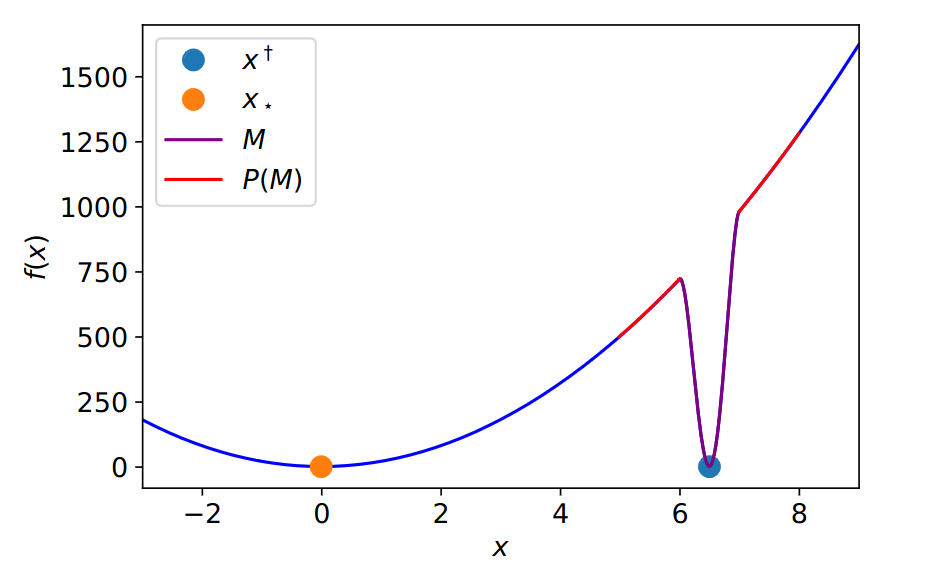
\includegraphics[scale=0.2]{lemma1}
\end{figure}

\begin{theorem}\label{thm1}
    Let $C_l$ be the set of functions sudh as $f$ is 
    $L$-smooth and $\mu_\ast$-OPSC with respect to the 
    global minima $x_\ast$ except n a region $M$ that 
    contains local minima $x^\dagger$ and satisfies \cref{lma1}.
    \begin{itemize}
        \item Gradient descent initialized randomly inside $M$ 
        with kearning rate $\gamma < \frac{\mu^\dagger}{L^2_{\mathrm{global}}}$
        converges to $x^\dagger$ almost surely.
        
        \item Gradient descent initialized randomly in 
        arbitary set $W: \mathcal{L}(W) > 0$ 
        with learning rate $\frac{2}{\mu^\dagger} < gamma \leq \frac{\mu_\ast}{L^2}$
        converges to $x_\ast$ almost surely.

    \end{itemize} 

\end{theorem}
\begin{proof}
    
\end{proof}

\begin{lemma}\label{lma2}
    Take gradient descent initialized randomly in set $W$ 
    with learning rate $\gamma \leq \frac{1}{2L}$.
    Let $X \subset \mathbb{R}^d$ arbitary set of points in 
    the landscape, $f$ is $L$-smooth over 
    $\mathbb{R}^d \setminus X$. Probabilty of encountering 
    any point of $X$ in first $T$ steps of gradient descent is 
    at most $2 ^ {(T + 1)d} \frac{\mathcal{L}(X)}{\mathcal{L}(W)}$.
\end{lemma}
\begin{proof}
    
\end{proof}

\begin{theorem}\label{thm2}
    Let $X$ be an arbitary set of points, 
    $f$ is $\mu_\ast$-OPSC with respect to a minima 
    $x_\ast \notin X$ over $\mathbb{R}^d \setminus X$.
    Let $c_X := \inf \left\{ \| x - x_\ast \| \:|\: x \in X  \right\}$
    and $r_W := \sup \left\{ \| x - x_\ast \| \:|\: x \in W \right\}$.
    The probabilty of not encountering ant points of $X$ during 
    gradient descent with learning ratee $\gamma \leq \frac{\mu_\ast}{L^2}$
    is at least $1 - \frac{r_W}{c_X}^{\frac{-d}{\log_2(1 - \gamma \mu_\ast)}} \frac{\mathcal{L}(X)}{\mathcal{L}(W)} 2^d$
    if $c_X \leq r_W$ and $1$ otherwise.
\end{theorem}

\begin{proof}
    
\end{proof}

\section*{Proposition}
Take the case of SGD 
$$ 
x_{t + 1} := x_t - \gamma \left( 
    \nabla f(x_t) + \xi_t
\right),
$$
where $\xi_t$ considered to be $\mathrm{Uniform}(-\sigma, \sigma)$.

\begin{proposition}
    Consider SGD on the function from figure \ref{fig:func}, 
    starting close to $x^\dagger$.
    If the learning rate is sufficiently small the iterations
    will never converge to $x_\ast$ nor to a small region around it, 
    regardless of the magnitude of the noise. 
    If the learning rate is large enough and stochastic noise
    satisfies certain bounds, SGD will converge to $x_\ast$ 
    from any starting point.
\end{proposition}

\begin{proof}
    
\end{proof}

\bibliographystyle{alpha}
\bibliography{sample}

\end{document}